\documentclass{beamer}
\usepackage[british]{babel}
\usepackage[utf8]{inputenc}
\usepackage{styles/jyumacros}
\usepackage[version=4]{mhchem}
\usepackage{textgreek}
\usepackage[absolute,overlay]{textpos}
\usefolder{styles}
\usetheme{jyu}

%change these to your own logos if needed (try and match sizes, otherwise, change sizes in Outer Theme file).
\titlegraphic{assets/coverlogo.pdf} %logo on the cover page
\newcommand{\smalllogo}{assets/small_white.pdf} %small logo on frames

%Personal info---------------------------------------------
\title{MARA-LEB}
\subtitle{An Insight into Nuclear Physics Experiments}
\date{20.8.2021}
\author[auth]{Jorge Romero}
\institute[inst]{University of Liverpool, Jyväskylän Yliopisto}
%----------------------------------------------------------

\begin{document}
\begin{frame}
\titlepage
\end{frame}

\begin{frame}{JYFL Acclab}
    \centering
    \vspace*{4em}
    \hspace*{-3em}
    \includegraphics[scale=0.6]{assets/JYFL}
    \vfill
    \begin{textblock*}{0.3\paperwidth}(.7\paperwidth,.5\paperheight)
        \includegraphics[scale=0.07]{assets/JYFL_locator}
    \end{textblock*}
    \begin{textblock*}{0.7\paperwidth}(0.01\paperwidth,.8\paperheight)
        \color{white}{The northernmost accelerator laboratory in the world!}
    \end{textblock*}
\end{frame}

\begin{frame}{About Me}
    \begin{textblock*}{0.5\paperwidth}(0.05\paperwidth,.25\paperheight)
        \begin{itemize}
            \item Bachelor Degree in Physics at the University of Valencia (Spain)
            \item Master's Degree in Nuclear Physics at the University of Sevilla (Spain)
            \item Dual Doctoral Student at the University of Liverpool and the University of Jyväskylä (Finland)
            \item \alert{Outside of Physics}: I play basketball, I love videogames and I am interested in many fields of knowledge.
        \end{itemize}
    \end{textblock*}
    \begin{textblock*}{0.3\paperwidth}(0.56\paperwidth,.15\paperheight)
        \includegraphics[scale=0.3]{assets/foto}
    \end{textblock*}
\end{frame}

\begin{frame}{A Nuclear Physics Experiment}
    \vspace*{-4em}
    \begin{itemize}
        \item<1-| alert@1> Accelerate something (beam)
        \item<2-| alert@2> Crash it into something else (target)
        \item<3-| alert@3> See what happens (detectors)
    \end{itemize}
    \begin{textblock*}{\paperwidth}(0\paperwidth,.45\paperheight)
        \centering
        \onslide<1>{\color{primary}{K130 Cyclotron at JYFL}}
        
        \includegraphics<1>[scale=0.2]{assets/K130}
    \end{textblock*}
    \begin{textblock*}{\paperwidth}(0\paperwidth,.45\paperheight)
        \centering
               
        \includegraphics<2>[scale=.7]{assets/beamtarget}
    \end{textblock*}
    \begin{textblock*}{\paperwidth}(0\paperwidth,.45\paperheight)
        \centering
        \onslide<3>{\color{primary}{The JUROGAM Ge-detector array}}
           
        \includegraphics<3>[scale=.117]{assets/juro}
    \end{textblock*}
\end{frame}

\begin{frame}{Nuclear Chart}
    \centering
    \hspace*{0.65em}
    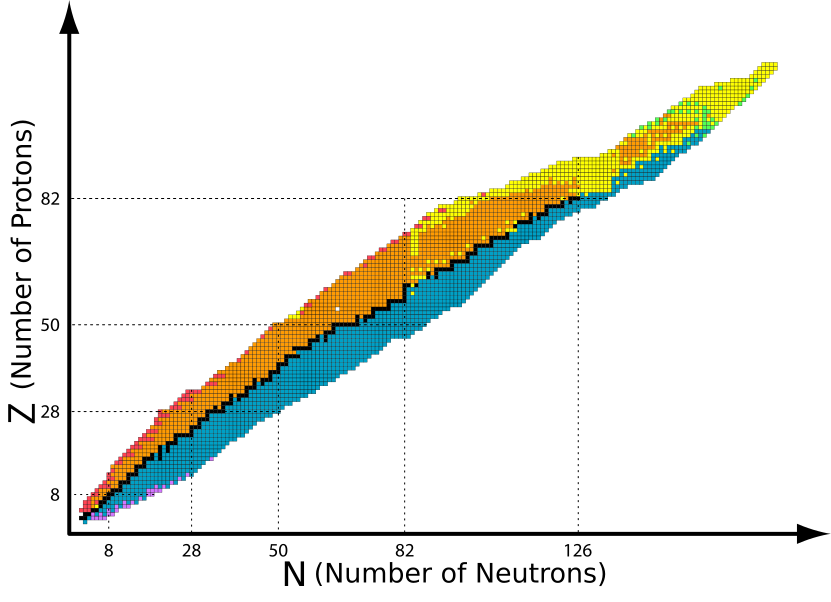
\includegraphics[scale=0.53]{assets/chart}
    \begin{textblock*}{0.1\paperwidth}(0.8\paperwidth,0.4\paperheight)
        \includegraphics[scale=0.5]{assets/legend}
    \end{textblock*}
\end{frame}

\begin{frame}{Reactions}
    \begin{textblock*}{1\paperwidth}(0\paperwidth,0.2\paperheight)
        \begin{center}
            \onslide<1>{Fusion: $a+A\longrightarrow B$}

            \vspace*{3em}
            \includegraphics<1>[scale=0.1]{assets/Fusion}
        \end{center}
    \end{textblock*}
    
    \begin{textblock*}{1\paperwidth}(0\paperwidth,0.2\paperheight)
        \begin{center}
            \onslide<2>{Fission: $a+A\longrightarrow B+C\ (+x)$}

            \vspace*{3em}
            \includegraphics<2>[scale=0.1]{assets/Fission}
        \end{center}
    \end{textblock*}

    \begin{textblock*}{1\paperwidth}(0\paperwidth,0.2\paperheight)
        \begin{center}
            \onslide<3>{Fusion-Evaporation: $a+A\longrightarrow B+x$}

            \vspace*{3em}
            \includegraphics<3>[scale=0.09]{assets/Fuseva}
        \end{center}
    \end{textblock*}
\end{frame}

\begin{frame}{MARA}
\vspace{4em}
The Mass Analysing Recoil Apparatus (MARA) uses electric and magnetic fields to select specific recoils from fusion-evaporation reactions.

\begin{center}
    \hspace*{-1em}
    \includegraphics[scale=0.65]{assets/MARA}
\end{center}
\end{frame} 

\begin{frame}{MARA-LEB}
    \vspace{4em}
    The MARA Low Energy Branch (MARA-LEB) will be used for exotic cases to suppress background.

    It will use \alert{laser ionisation} for both measurement and purification.
    
    \begin{center}
        \hspace*{-2em}
        \includegraphics[scale=0.8]{assets/LEB}
    \end{center}
\end{frame} 

\begin{frame}{MARA-LEB}
    \begin{textblock*}{0.65\paperwidth}(0.05\paperwidth,0.25\paperheight)
        MARA-LEB is of interest in the N=Z region, close to the proton \alert{dripline}, where no more protons can be added to the nucleus.
    \end{textblock*}

    \begin{textblock*}{0.54\paperwidth}(0.05\paperwidth,0.42\paperheight)
        \ce{^{80}Zr}, \ce{^{94}Ag} and \ce{^{100}Sn} and their neighbours are of particular interest.
    \end{textblock*}

    \begin{textblock*}{0.8\paperwidth}(0.2\paperwidth,0.15\paperheight)
        \begin{center}
            \hspace*{-1em}
            \includegraphics[scale=0.65]{assets/ROI}
        \end{center}
    \end{textblock*}
\end{frame}

\begin{frame}{Simulations - Ion Transport System}
    \vspace*{2em}
    \centering
    \includegraphics<1-2>[scale=0.1]{assets/Simion}
    \includegraphics<3>[scale=0.4]{assets/bendstraight}
    \includegraphics<2-3>[scale=0.4]{assets/simu}
\end{frame}

\begin{frame}{SEMF}
    \centering
    \vspace*{3em}
    \alert{\textbf{Society for Multidisciplinary and Fundamental Research}}

    "SEMF aims to establish a pluralistic community of scientists, creatives, academics, artists, students, intellectuals and, generally, enthusiasts united under the common goal of delving deeper into fundamental questions."

    \vspace*{1em}
    \includegraphics[scale=0.1]{assets/semf_logo}
    
    \vspace*{1em}
    \url{http://semf.org.es}

\end{frame}

\end{document}